 \documentclass[french]{article}
 \usepackage{setspace}
% \onehalfspacing
 \usepackage[utf8]{inputenc}
 \usepackage[T1]{fontenc}
 \usepackage{lmodern}
 \usepackage[a4paper]{geometry}
\usepackage[french]{babel}
\usepackage{wallpaper}
 \usepackage{graphicx} %images
 \usepackage{graphics} %images
 \usepackage{textcomp}
 \usepackage{multicol} %utiliser l'environnement\begin{multicols}{2} 
 %ou sur grande page pour inclure flotants l'option \twocolumn[titre1colonne]{textedeuxcolonnes}
\usepackage{microtype}
 \usepackage{geometry}
 \usepackage{fancyhdr}
 \usepackage{array}
 \usepackage{multirow}
 \usepackage{float}
\usepackage{tocloft}  %table des figures
 \usepackage{hyperref}
 \usepackage{indentfirst} %indentation des paragraphes en debut de section
 \usepackage{amsmath,amsfonts,amssymb} %équations, matrices etc...
 \usepackage{cell} %bibliography style
 \geometry{vmargin=2.5cm, hmargin=2cm}
 \hypersetup{colorlinks=true, linkcolor= black, citecolor=black} %gestion lien hypertexte
 \usepackage{lscape}   % paysage
 \usepackage{pdflscape,array,booktabs}%pages du pdf avec tableau en paysage
 \usepackage{cite} %citations multiples
 
 \newcommand{\auth}{Clément Viguier}
 \newcommand{\tlte}{Strategy Space}
  
%Césures:
\hyphenation{tou-che trou-bles trou-ble ima-ge ima-ges étu-des étu-de non-con-ven-tion-nelle}
 %__________________________________________________________
 \newenvironment{changemargin}[2]{\begin{list}{}{%
 \setlength{\topsep}{0pt}%
 \setlength{\leftmargin}{0pt}%
 \setlength{\rightmargin}{0pt}%
 \setlength{\listparindent}{\parindent}%
 \setlength{\itemindent}{\parindent}%
 \setlength{\parsep}{0pt plus 1pt}%
 \addtolength{\leftmargin}{#1}%
 \addtolength{\rightmargin}{#2}%
 }\item }{\end{list}}
 
 
 % titre du document
 \title{\tlte}
 % auteur du document
 \author{\auth}
 
 \begin{document}
 \pagestyle{fancy}
 \fancyhead[R]{\small\auth}
 \fancyhead[L]{\small\tlte}
 \renewcommand\headrulewidth{0.5pt}
 \thispagestyle{empty}
 
 \newpage
% \strut
% \ThisLRCornerWallPaper{1}{figure/frpage.pdf}
% \newpage
% 

 \begin{titlepage}
 
 \maketitle
 \centering
 
 \thispagestyle{empty}
 \end{titlepage}
 
 

%--------------------------------------------
% \begin{changemargin}{2cm}{2cm}
% \vspace*{2cm}
% \thispagestyle{empty}
% \tableofcontents
%\thispagestyle{empty} 
% \end{changemargin}
%\newpage

%--------------------------------------------
% \begin{changemargin}{2cm}{2cm}
% \vspace*{2cm}
% \thispagestyle{empty}
%\listoffigures
%\thispagestyle{empty} 
% \end{changemargin}
%\newpage

%%--------------------------------------------
% \begin{changemargin}{2cm}{2cm}
% \vspace*{2cm}
% \thispagestyle{empty}
%\section*{Table des abréviations}
%\begin{enumerate}
%\item SLA : Species Leaf Area
%
%
%\end{enumerate}
%\thispagestyle{empty} 
% \end{changemargin}
%--------------------------------------------

\newpage

%
%
% \setcounter{page}{1}
% \begin{bf}
% \paragraph{Résumé}
% \indent \end{bf}
% 
%\newpage
%~
%\thispagestyle{empty}
% \newpage


%--------------------------------------------
 \twocolumn{
 \section{Introduction}
%Pourquoi un modèle mécanistique ?\\
%Quels processus ?\\
%Comment différencier les espèces par types fonctionnel/stratégies ?\\
%Quels sont les compromis entre stratégies ?\\

L'utilisation de la modélisation permet de questionner les dynamiques des communautés en dépassant les contraintes de complexité d'un système réel. Cela nécessite la définition d'un cadre conceptuel solide permettant de reproduire ces dynamiques grâce à l'intégration des mécanismes moteurs et structurants. L'étude des communautés et des interactions inter- et intra-spécifiques nécessite la construction de systèmes stables non dominés par des super-espèces. Ce besoin est soutenu par le concept de compromis qui établit qu'une espèce ne peut être compétitive sur tous les aspects du développement végétal. Ces compromis contraignent les espèces à faire des choix de développement et ainsi définir des stratégies de conservation. Afin de mieux comprendre la coexistence des espèces et les structures et dynamiques des communautés, de nombreux cadres conceptuels ont été développés. Ceux-ci ont pour ambition de définir des types fonctionnels selon un nombre limité d'axes de différenciation et de cerner les mécanismes principaux de contrôle des communautés. La difficulté de la définition d'un tel cadre réside dans le choix des axes. Ces axes doivent à  la fois être suffisamment nombreux pour délimiter les différents types fonctionnels et rendre compte de la diversité des stratégies observées, et en nombre relativement réduit afin de permettre l'étude théorique de la communauté. Au delà du nombre d'axes, la pertinence des axes choisis est cruciale. Ces choix sont sujet à discussion, dépendant des questions posées et du système considéré. Je présente ici quelques espaces de stratégies explicites ou implicitement développés au travers de modèle de simulation.

\section{Revue des espace de stratégies existants}
\subsection{Espace CSR de Grime}
En 1977, Grime \cite{Grime1977} décrit un espace de stratégie à deux dimensions : stress - perturbation. Il définit le stress comme une contrainte externe limitant la production de biomasse. La perturbation est décrite comme un processus de limitation de la biomasse végétale par destruction.\\
\indent En considérant les valeurs extrêmes de ces deux axes, on peut distingué 4  permutations possibles : fort stress-forte perturbation, fort stress-faible perturbation, faible stress-forte perturbation et faible stress-faible perturbation. Grime avance que l'association fort stress-forte perturbation ne permet pas la réinstallation d'un peuplement après une perturbation. Il distingue donc trois stratégies dominantes dans chacune des positions viables dans l'espace ainsi défini (figure \ref{fig:Grime}). Dans un contexte de faible pression environnementale (faible stress et perturbation) la fertilité est importante et les opportunités de croissance ouvertes pour une grande diversité de végétaux. Cela se traduit par une forte compétition inter-spécifique, et la stratégie dominante est celle qui permet l'émergence des semis malgré des conditions de faible disponibilité. Si le stress est important, la stratégie dominante est celle qui favorisera la tolérance au stress au détriment des capacités de reproduction et ou d'un développement rapide.\\

 \begin{figure}[H]
 \centering
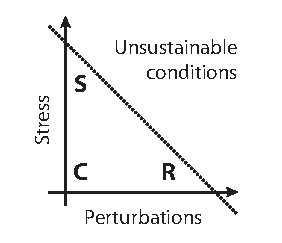
\includegraphics[width=\columnwidth]{Grime_triangle.pdf}
 \caption{Triangle de Grime.}
\label{fig:Grime}
\footnotesize{Espace stratégique à deux dimensions : stress-perturbations. L'accumulation stress-perturbations ne permet pas le maintien de végétation. C : espèces compétitives, R : espèces rudérales, S : espèces tolérantes au stress.}
 \end{figure}

\indent Cependant, l'utilisation de concept aussi larges que le stress et la perturbation, constitue à la fois une force et une faiblesse de ce cadre conceptuel. En effet, ces définitions sont applicables à des systèmes très variés (au delà même du monde végétal) et la classification en différentes stratégies selon ces axes peut être universellement utilisée. Cependant il est évident que les formes de stress (eau, nutriments, température...) et de perturbation (chute d'arbre, feu, pâture...) diffèrent d'un système à l'autre. Les critères de compétitivité et de résistance au stress sont donc dépendants des conditions abiotiques et des autres compétiteurs du système considéré. Ainsi, des stratégies similaires entre deux systèmes ne peuvent être traduites en caractéristiques (traits fonctionnels) similaires. Réciproquement, il est impossible d'établir un lien direct entre traits fonctionnels et stratégies.\\
\indent Cette difficulté de mettre en relation ce cadre théorique puissant et les traits fonctionnel constitue un obstacle majeur à son utilisation.\\

%
%2 dimension. Une permutation ignorée car ne permettant pas la recolonisation.
%cadre conceptuel fort pour la compréhension des écossytèmes. Groupes fonctionnels explicites. Mais pas de lien avec les traits fonctionnels.
%Définition à base de concept (stress, compétition). Définition dépendante de l'environnement. too simple
\subsection{L'espace LHS de Westoby}
Le triangle de Grime fait référence dans la définition des types fonctionnels structurant les communautés. Cependant, Westoby met en lumière la difficulté de son utilisation et son incapacité à expliquer/illustrer certains motif \cite{Westoby1998}. Selon Westoby un espace de stratégies doit avoir pour vocation de : (1) exprimer des différences pertinente de comportement entre espèces, (2) permettre le positionnement d'une plante par connaissance seule de ces caractéristiques (et non son positionnement au sein d'un environnement), (3) utiliser comme axes des traits uniques suffisamment accessibles, (4) capturer les variations des autres traits fonctionnels grâce à des relations de corrélation entre les axes et les traits non détaillés.\\
\indent A partir de ces critères il définit un espace de stratégies à trois dimensions : Specific Leaf Area (L) - hauteur à maturité (H)- masse des graines (S). La SLA élevée permet un retour sur investissement de la masse sèche produite très rapide. Au contraire une réduction de la SLA réduit cette rentabilité, mais elle est compensée par une durée de vie plus grande (grâce à un investissement dans la résistance structurale ou chimique). Une forte SLA peut être associée à des stratégies de production précoce de feuilles et un turnover important, avantageux dans un environnement fortement compétitif. La longévité accrue associée à une faible SLA permet une meilleure efficacité photosynthétique et un stockage d'azote plus important, constituant un avantage face au stress. Cet axe peu donc être perçu comme une transcription de l'axe CS du triangle de Grime \cite{Grime1977}. Les traits S et H traduisent la résistance aux perturbations déjà considérée dans le cadre théorique de Grime (axe R). La taille à maturité traduit selon Westoby la capacité à prendre la tête (et éventuellement gagner) la course à la lumière pouvant intervenir lors de perturbations de l'environnement. La masse des graines est représentative du compromis entre augmentation des chances de survie (grosses graines) et augmentation des opportunités (nombreuses petites graines). Cette décomposition est cependant discutable. En effet, la hauteur à maturité est signe d'un investissement fort qui peut représenter une grosse perte dans un environnement sujets à perturbations (feu, pâtures, épisodes de gels...) ou au contraire une forme de résistance (espèces ligneuses moins sujettes à la pâture, tissus protecteurs).

%3 dimmensions, à discuter
%Retranscript le CSR avec les traits fonctionnel. Non dépendant de la connaissance de la communauté. Construire pour une utilisation globale. Mais traits non stables. Ne transcript pas assez la diversité des stratégies. = manque de dimensions.

\indent L'espace des stratégies défini par Westoby permet le positionnement simple de toute espèce grâce à des traits fonctionnels accessibles. Cependant, bien que l'auteur explique que les autres traits fonctionnels peuvent être accessible par connaissance des corrélation avec les axes utilisés, établir ces relation n'est pas pour autant simple. Le manque de relations fonctionnelles ou corrélatives entres les traits ne permet pas la définition de types fonctionnels suffisamment variés.\\
\indent De plus, la plasticité des traits (SLA par exemple) implique que leur capacité de caractérisation des espèces est limitée dans l'espace et le temps, dans la mesure où des changements de conditions (géographique ou temporelles) entrainent des changements de valeurs des traits. En plus de ne pas permettre l'utilisation de ce cadre théorique en modélisation prédictive qui, par essence, modifie les conditions modélisées, cette limite s'oppose aux objectifs d'utilisation universelle visés par Westoby \cite{Westoby1998}.\\
\indent Les modèles de simulation de dynamiques de végétation ont pour objectif de représenter les dynamiques des communautés de végétaux et leur compositions en termes de groupes fonctionnels. En ce sens ils ne représentent pas des espèces, mais des groupes rassemblant des caractéristiques communes et donc ayant un rôle identique dans l'organisation de la communauté. La volonté de représenter la diversité des comportements et des stratégies (dans la diversité des biomes) nécessite de considérer des axes de différenciation plus nombreux que les cadres théoriques précédemment cités. Leur étude peut permettre la mise en évidence des axes de stratégies considérés.

\subsection{Modèle de la famille Kleidon}

\indent Les modèles de dynamique globale modélisent les espèces par le biais des traits fonctionnels. L'étude de ces traits et des compromis associés peut permettre de dégager des axes de différenciations pertinents. Cette étude portera sur l'importance de la variabilité des mécanismes considérés, la stabilité des traits et les contraintes ou corrélations entre les traits.\\

\indent Ces modèles sont représentés principales par le modèles de Kleidon et Mooney, et ses dérivés \cite{Kleidon2000, Reu2010, Pavlick2013}. Les différents traits fonctionnels caractéristiques des espèces sont listés dans la table \ref{tab:comp_traits}. Le modèle développé par Kleidon et Mooney rassemble 12 traits fonctionnels, dont les corrélations sont étudiées plus en détails par Reu et al.\cite{Reu2010}. Le modèle JeDi-DGVM \cite{Pavlick2013} ajoute 3 nouveaux traits au 12 précédemment considérés, afin d'inclure une température critique et le renouvellement tissulaire (en complément de la sénescence pour la biomasse active).\\

Il est possible de regrouper les traits considérés en traits d'allocations (t5, t6, t7, t8, t9, t10), de tolérance aux conditions météo (t1, t2, t4, t11, t13), d'efficacité (t12), de  reproduction (t3) et de renouvellement tissulaire (t14, t15).\\
\indent Les traits d'allocation peuvent également être regroupés en trois axes : développement, stockage et reproduction.
Le développement végétal est lui même décomposé selon deux axes : aérien(t6, t9)-souterrain(t7, t10) et structure(t9, t10)-actif(t6, t7). Il y a ici deux trade-offs importants : le compromis entre l'acquisition de ressources souterraines (eau, nutriments) et la production de matière organique (photosynthèse), et le compromis entre la durée de vie (et éventuellement de la résistance) et la production de tissu actif. De tels compromis fonctionnels internes (résultant de mécanismes internes de partitionnement des ressources) sont fondamentaux. Cependant investir majoritairement à l'extrémité de l'un des axe ne peut pas réellement constituer une stratégie viable car entrainerait un déséquilibre fonctionnel. De plus, si une diversité de rapports des tissus structurels:tissus actifs est possible, là encore un équilibre est primordial pour l'intégrité de la plante. Cette idée d'équilibre est explorée par des modèles basés sur l'équilibre fonctionnel ou le partitionnement optimal des ressources \cite{Maire2009,Lohier2014}. Cette hypothèse est soutenue par l'observation de changement d'allocation entre tige, feuilles et racines étudié par Poorter et al. \cite{Poorter2012}. Ils ont mis en évidence des transitions d'allocation en réponse à des changements de conditions (disponibilité en eau, en nutriment, rayonnement, température...). Ces résultats suggèrent la plasticité des traits d'allocation. Cela pose la question de l'existence de traits de contrôle, intrinsèques et spécifiques qui déterminerait véritablement la stratégie de l'espèce. De même, l'étude de corrélation des traits \cite{Reu2010} ne mets pas en évidence une corrélation négative forte (-0.34) entre t6 (croissance aérienne) et t7 (croissance souterraine), renforçant l'idée qu'un compromis d'allocation entre compartiment aérien et compartiment souterrain n'est pas nécessaire. Dans la même étude on note la forte stabilité des traits (t5 à t8) entre les biomes et au sein d'un même biome, suggérant là encore que l'allocation des ressources dans le développement n'est pas un axe de différenciation fort. Les fortes corrélations négatives (dans tous les milieux modélisés) entre les traits de développement et de stockage (t6 vs t8, t7 vs t8), entre les traits de développement et de reproduction (t6 vs t5), et entre les traits de stockage et reproduction (t8 vs t5), sont elles marqueurs d'une différenciation stratégique plus importante.\\
\indent Les traits de tolérance aux conditions météo (t1, t2, t4, t11, t13) comprennent le contrôle de la sénescence et les temps de réponse aux changements de conditions. Ces paramètres contrôlent la force (t11) et la vitesse de réponse (t1, t2, t4, t13). Cette notion de réactivité est importante mais les contreparties ne sont pas évidentes. Une mémoire plus longue suppose peut être désavantageuse lors du retour de bonnes conditions de croissance, et désavantageuse lors d'une aggravation des conditions. Estimer l'impact de la réactivité reviens donc à considérer l'importance relative entre un retard de croissance et le prolongement de la croissance dans de mauvaise conditions. Au delà de cette dualité, une faible réactivité (temps de réponse élevé) permet la stabilisation de la croissance dans le cas de conditions avec une forte variabilité temporelle. De la même façon un temps de réponse au conditions climatiques court entrainant une sénescence rapide est un avantage dans les milieux avec une faible variabilité temporelle des phénomènes météo.\\

\indent La masse des graines, axe de spécialisation majeur selon Westoby \cite{Westoby1998}, est marqueur des perturbations chroniques du milieux, a déjà été discutée et semble essentielle à la différenciation stratégique des espèces.\\

\indent La LUE ou Light Use Efficiency est également un trait caractéristique. Ce trait augmente la production brute de matière organique mais augmente le coût de la respiration.\\

\indent Les traits assimilés aux temps de renouvellement des tissus ne présentent pas d'avantages apparents. Ces traits permettent de rendre compte d'un phénomène observé mais leur intégration dans le modèle ne met pas en évidence un processus de différenciation stratégique. Mettre en lien ce renouvellement avec l'investissement en carbone structurel, ou avec un trait de résistance témoignerait d'une stratégie conservatrice. L'existence de relations entre ces traits et les traits de tolérances aux conditions, et plus généralement des traits de résistance, simplifierait l'établissement de l'espace de stratégie par l'intégration seulement d'un axe de résistance au stress comme suggéré par Grime. De telles relations sont à mettre en évidence avant de faire ce type de simplification.\\

\indent Les modèles présentés ci-dessus présentent des traits de spécialisations divers et capturent l'essentiel des processus biologiques de la vie d'une plante. On notera cependant que si les axes principaux des traits d'allocation peuvent être conservés (développement, stockage, reproduction), la décomposition compartiments aérien-souterrain et tissus structural-actif n'est pas évidente. Une alternative à cette décomposition est la théorie de l'équilibre fonctionnel implémenté par Maire et Soussana \cite{Maire2009,Soussana2012}, discutée dans la suite du manuscrit.



\subsection{Modèles d'équilibre fonctionnel}
L'équilibre fonctionnel permet de contourner la question du paramétrage de l'allocation entre feuilles et racines et faisant l'hypothèse que le partage des ressources est optimal pour la maximisation du taux de croissance. Cette hypothèse, explique des changements d'allocation en fonction de la disponibilité en ressource \cite{Osone2005}. Cette hypothèse semble raisonnable dans la mesure où une utilisation non optimale des ressources constituerait un désavantage compétitif. Le carbone est distribué entre feuilles et racines de façon à ce que l'influx racinaire comble exactement la demande pour la production de matière organique par les feuilles (figure \ref{fig:equilibre}). Ce mécanisme permet d'éviter une allocation trop importante dans les feuilles non soutenue par l'activité racinaire, ou au contraire un influx racinaire trop important par rapport au besoins foliaires. Lohier met en évidence des équilibres d'allocation (aérien-souterrain) différents contrôlés par des efficacités photosynthétique et d'absorption différentes \cite{Lohier2014}. Il n'y a cependant pas dans le modèle de Lohier de contrepartie à une efficacité photosynthétique plus importante. Cette efficacité photosynthétique est à rapprocher de la LUE. Ainsi, il parait naturel d'associer cette efficacité avec un taux de respiration plus important.\\
\indent L'efficacité d'utilisation d'une ressource est un concept intéressant, mais il est difficile de répondre à la question du coût de cette efficacité. \\

\begin{figure*}
\centering
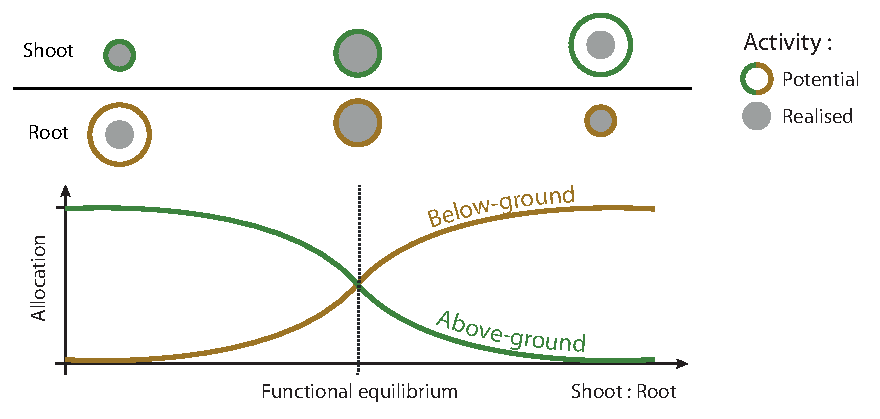
\includegraphics[width=0.8\textwidth]{equilibrium.pdf}
\caption{Allocation plastique et l'équilibre fonctionnel.}
\label{fig:equilibre}
\footnotesize{Représentation de l'équilibre fonctionnel et de la plasticité d'allocation entre compartiments aériens et souterrains. Les cercles verts et oranges représentent respectivement l'activité potentielle du compartiment aérien et du compartiment racinaire (en relation avec la biomasse de chaque compartiment). Les disques grisés indiquent l'activité réalisée. La position centrale est celle de l'équilibre fonctionnel où les activités aérienne et souterraine sont à l'équilibre. Dans le cas d'une activité aérienne réalisée inférieure à l'activité potentielle, l'allocation vers les racines est privilégiée.}
\end{figure*}
  

 
%
%\indent Coordination photosynthétique : équilibre entre carboxilation et flux d'électrons (pour une luminosité et une concentration en carbone donnés). A mettre en relation avec l'efficacité d'utilisation de l'azote. Définition d'une LNC optimale (conditionnel). Qu'est-ce que cela implique sur l'équilibre pour l'azote et le carbone entre machinerie cellulaire et croissance structurale ? Distinction entre partionnement carbone-azote pas claire.\\
%contourner les problème d'allocation ou de traits fonctionnels variables par des hypothèses d'équilibre fonctionnel : entre tige et racines, entre croissance et efficacité (photosynthèse coordonnées, voir dans thèse de Vincent Maire)

\subsection{Autres modèles}
D'autres modèles ont été développés pour répondre à différentes problématiques et apportent des alternatives différentes.\\

\indent Suite à une revue des modèles de prairies existants \cite{Taubert2012}, Taubert développe le modèle Grassmind \cite{Taubert2014} avec pour objectif d'étudier la relation diversité-productivité des prairies cultivées. Le modèle présente un compromis d'allocation entre trois compartiments : la tige, les racines et les graines. La ressource consacrée à la reproduction n'est allouée que si les conditions sont favorables, sinon elle est partagée entre les deux premiers compartiments. Le stockage et les mécanismes de résistance ne sont pas pris en compte. La différenciation stratégique des espèces est très détaillée sur l'aspect reproduction et recrutement (4 paramètres), et la sénescence et mortalité (durée de vie des feuille, des racines, des individus et mortalité des graines). L'efficacité photosynthétique est également un trait spécifique à l'espèce, mais aucune contrepartie explicite à une forte productivité n'est intégrée. La symbiose racinaire et la capacité à fixé l'azote est également un axe de différenciation. Là encore l'idée d'efficacité des compartiments aérien et souterrain est intégré, mais les contreparties sont absentes.\\

\indent Dans le modèle Lingra Schapendonk et collaborateurs \cite{Schapendonk1998} utilisent une approche puits-source pour modéliser la productivité d'une espèce : Lolium perenne. Cette approche est intéressante car intègre l'équilibre entre feuilles et racine de façon mécanistique. Cependant cet équilibre repose sur la capacité de croissance des feuilles, processus très détaillé et nécessitant une calibration exigeante. L'intérêt de l'approche puits-source est l'alternance entre les phases où l'apport est limité, entrainant la consommation des ressources stockées, et les phases où le besoin est limité (car taux d'élongation foliaire fixe) entrainant la reconstitution des réserves. Ici la plasticité d'allocation est gérée de façon mécaniste par le contrôle de l'élongation foliaire. La capacité de stockage de l'espèce est une caractéristique que l'on peut raisonnablement considérée spécifique à l'espèce.  L'efficacité potentielle de l'usage de la lumière (LUE) est également un paramètre déterminant dans le comportement du modèle et constituerait un axe de spécialisation si le modèle était paramétré pour plusieurs espèces. L'aspect mécaniste de cette approche est très intéressant, cependant l'effort de paramétrage nécessaire est ici important, notamment sur le taux d'élongation foliaire.\\

\indent Le modèle dynamique global de végétation développé par Scheitter et Higgins \cite{Scheiter2009}, comparable aux modèles de la famille Kleidon, a intégré l'idée d'une allocation adaptative. Les paramètres d'allocation contiennent des indicateurs des conditions environnementales (lumière et humidité) afin de favoriser la croissance du compartiment limitant la croissance de la plante. Cette adaptation est construite autour de valeurs spécifiques de l'espèce, et est limitée autour de ces valeurs par défaut grâce à un coefficient de déviation. Cette solution pourrait être une alternative à l'équilibre fonctionnel. De tels coefficient indicateurs des conditions environnementales permettent une réponse adaptative de la plante et permet de mimer les mécanismes d'adaptation encore méconnus. L'association à l'hypothèse de l'équilibre fonctionnel est intéressante et est explorée dans la suite de ce document.


\section{Définition d'un espace de stratégies}
Le choix des axes de différenciation stratégique est dépendant du système étudiée. Les modèles et cadres théoriques analysés s'intéresse à des système variés allant de la prairie monospécifique (Lingra \cite{Schapendonk1998}, Gemini\cite{Soussana2012}) jusqu'à des DGVMs considérant arbres, arbustes et herbes. Les traits fonctionnels descriptifs des espèces dépendent de la diversité des questions posées, du système considéré, du degré de détails et de complexité désiré et de phénomènes particuliers ayant un impact sur la structure du système. Afin de choisir les traits les plus adaptés à notre situation, nous tentons de définir les points précédents.

\subsection{Cas des prairies de montagne}
L'objet d'étude étant les prairie de montagne , plusieurs caractéristiques spécifiques se dégagent. Tout d'abord, la diversité des espèces considérées est réduit à l'ensemble des herbes, et ne comprend ni arbre ou arbuste. De ce fait, s'il n'est pas possible de retirer un trait de la liste des traits considérés jusqu'à maintenant, les intervalles de valeurs possibles pour chaque traits sont réduits (i.e. masse de la graine). Un autre élément important est la sévérité du milieu montagnard. Ce milieu est en effet caractérisé par un certaine aridité, des température basses, une luminosité élevé. La résistance des parties aériennes et souterraine et donc essentielle. 

\subsection{Prototype d'un espace de stratégies}
L'analyse des espaces de stratégies effectuée nous permet de définir des axes intéressant de différenciation stratégique.  L'utilisation des traits fonctionnels présente des intérêts pratiques incontestables \cite{Westoby1998}. Les traits proposés par Westoby ne permettent cependant pas de représenter la diversité des stratégies que l'on souhaite représenter et ne présentent pas la plasticité désirée. Idéalement les traits fonctionnels considérés seraient des traits intrinsèques invariants, qui contrôleraient les autres traits fonctionnels. L'identification de tels traits au travers de l'étude des modèles de végétation n'a pas été possible et dois être prolongée au travers de l'étude directe des traits fonctionnels. Les modèles de la famille Kleidon intègrent les processus d'intérêt et permettent l'ajout du cycle du carbone mais le système d'allocation peut être repensé pour intégrer le principe d'équilibre fonctionnel. Une liste de traits de différenciation stratégique est ici proposée comme base de travail et de réflexion. Les idées de compromis et contre-parties associés à chacun de ces traits sont ensuite discutées. Les 9 axes de différenciation retenus sont les suivants :

\begin{itemize}
\item efficacité photosynthétique,
\item efficacité d'absorption racinaire,
\item allocation pour le développement végétal,
\item allocation pour la reproduction,
\item allocation pour le stockage,
\item allocation pour la résistance,
\item réactivité,
\item masse des graines,
\item allométrie spatiale.
\end{itemize}

\indent Les efficacités des activités foliaire et racinaire constituent (1) le moteur de l'équilibre fonctionnel, (2) la contrainte entre le rapport masse de tissu actif:masse  de tissu structurel. Illustrons ces deux points en prenant l'exemple de la feuille. Une forte efficacité foliaire entraine un rendement plus important de l'activité photosynthétique, et donc un investissement en matière organique nécessaire plus faible. Cependant cette productivité a un cout, se traduisant par une fraction de la matière organique investie dans les tissus actifs supérieure à celle investie dans les tissus de structure, diminuant la durée de vie des feuilles et augmentant le coût carbone de la respiration.
\indent Le prototype présenté suggère un compromis d'allocation entre le développement végétal, le stockage de ressource, le développement de mécanismes de résistance et la reproduction. Les coefficients d'allocation pour chacun de ces compartiments peuvent être fixes ou, à l'image du modèle de Scheiter et Higgins \cite{Scheiter2009}, pourraient intégrer un caractère adaptatif permettant un glissement en fonction des conditions météorologiques ou du statut de la plante. Scheiter et Higgins utilisent cette adaptation des coefficients d'allocation pour la distribution des ressources entre feuilles, racines et tige. Il conviendrait de définir les drivers climatiques qui contrôlent l'équilibre entre développement végétal, stockage et reproduction pour mettre en place cette plasticité d'allocation. L'allocation aux mécanismes de résistance peut être contrôlée par ce genre de coefficients d'adaptation, mais la diversité des mécanismes de résistance (discutée dans le paragraphe suivant) rend complexe de telles considérations.

\indent Les phénomènes de résistance à des phénomènes particuliers (gel, pâture, rayonnement élevé...) sont rarement implémentés dans les modèles de végétation. Un phénomène fait exception, le feu, qui a un impact extrêmement fort sur la structure de certains écosystèmes (savanes, forêts...) \cite{Scheiter2013}. Dans cas, des traits particuliers sont identifiés comme la densité du bois, la biomasse de l'écorce, pour quantifier cet investissement dans la résistance au feu. Malheureusement, la complexité et la diversité des mécanismes de défense ou de résistance déployés par les plantes n'est pas toujours accessible, et est difficile à implémenter (surtout en considérant un nombre réduit de traits). Si l'on souhaite cerner plus de mécanismes de résistance avec un seul coefficient, soit on suppose que les mécanismes de résistance n'ont pas d'effet spécifique, soit on ne considère qu'un seul de ces mécanisme a un impact dans un écosystème donné (autrement dit, plusieurs phénomènes perturbateurs ne peuvent avoir un impact de même amplitude sur cet écosystème). Ce carbone investi dans les mécanismes de résistance, associé avec une allocation plastique contrôlée par les conditions (similaire à l'allocation plastique proposée par Schieter et Higgins \cite{Scheiter2009}) permettrait de mimer les phénomènes de plasticité des traits observée par exemple dans le cas d'évènements de sécheresse courts \cite{Jung2014}. En effet, une allocation privilégiée dans le "carbone de résistance" (sans croissance foliaire) augmenterait la LDMC et diminuerait la SLA comme observé par Jung \cite{Jung2014}. Par simplification les mécanismes de résistance peuvent être directement lié à la fraction de carbone structural. \\

\indent La reproduction dans les modèles DGVMs est amorcée dès que les conditions sont favorables, de même pour la germination. Dans ces modèles, la maturité des plantes (ou graines) n'est pas prise en compte. Au contraire, Taubert \cite{Taubert2014} intègre 3 traits spécifiques aux espèces (et 2 non spécifiques) pour décrire le recrutement et l'émergence de la descendance. Ce contraste pose la question du réel impact de ces traits sur la capacité des espèces à se propager. Les traits considérés sont : l'intervalle de temps entre le semis et la germination, le taux de germination et l'age de maturité sexuelle. Il semble raisonnable de penser que les 2 premiers traits, s'il ne peuvent être ignorés, peuvent être estimés à partir de la masse de la graine et/ou des conditions environnementales. La question de la maturité sexuelle, et de l'ajout d'un trait associé, reste ouverte.\\

\indent L'utilisation d'un seul paramètre pour rendre compte de plusieurs mécanismes nécessite des hypothèses fortes. Dans le cas de la réactivité, ou de la prise de risques, les mécanismes mis en jeu sont la vitesse de réaction à un changement de conditions et l'amplitude de la réaction, mais les dimensions augmentent lorsque l'on considère plusieurs ressources indépendamment (eau, lumière, carbone, azote...). Considérer un seul paramètre revient donc à faire la première hypothèse suivante : si une espèce à un comportement conservateur pour une ressource, alors il en est de même pour les autres ressources. Autrement dit, une espèce ne peut avoir une réponse risquée face à un changement de la disponibilité en eau d'une part, et une réaction modérée face à un changement de la disponibilité en radiation actives. Le deuxième problème posé par cet unique paramètre est la relation entre temps de réponse et amplitude de la réaction aux changements de conditions. Face à ce problème soit on considère que la force de la réaction n'est pas spécifique à l'espèce, soit on on cherche une relation entre temps de réaction et force de réaction, soit on introduit un trait supplémentaire.\\

\indent Le compromis de croissance spatiale, entre la croissance en hauteur (ou profondeur) et la croissance en largeur, permet de distinguer les espèces favorisant l'étalement et réduisant l'auto-ombrage, et les espèces favorisant la croissance en hauteur et l'accès à la lumière en milieu compétitif. Ce trait contrôle le compromis entre la hauteur à maturité et la densité des tiges pour le cas particulier des prairies \cite{Maire2013}.


\section{Conclusion}

%--------------------------------------------
% \begin{figure}[H]
% \centering
%\includegraphics[width=\columnwidth]{path/name.ext}
% \caption{Caption}
%\label{demyelin}
%\footnotesize{Caption - details}
% \end{figure}

%--------------------------------------------
%\begin{figure*}
%\centering
%\includegraphics[width=0.8\textwidth]{path/name.ext}
%\caption{Caption}
%\label{relaxation}
%\footnotesize{Caption - details}
%\end{figure*}
%  

%--------------------------------------------
 \nocite{TitlesOn}
 \bibliographystyle{cell}
 \bibliography{PESS}
 
 
 
\begin{landscape}
\appendix

\begin{table}[htbp]
  \centering
  \caption{Table des traits fonctionnels considérés dans les modèles de la famille Kleidon.}
    \begin{tabular}{rrrrrr}
    \toprule
          & N° & \multicolumn{2}{c}{Authors} & \multicolumn{1}{c}{Cost} & \multicolumn{1}{c}{Benefits} \\
          &       & \multicolumn{1}{c}{Kleidon \& Mooney - Rue} & \multicolumn{1}{c}{Pavlick} &       &  \\
    \midrule
    \multicolumn{1}{l}{Date} &       & \multicolumn{1}{c}{2000 - 2011} & \multicolumn{1}{c}{2013} & \multicolumn{1}{c}{-} & \multicolumn{1}{c}{-} \\
    \midrule
    \multicolumn{1}{l}{Traits} & \multicolumn{1}{l}{t1} & \multicolumn{1}{l}{growth response time to moisture} & \multicolumn{1}{l}{growth response time to moisture} & \multicolumn{1}{l}{lesss time for C assimilation} & \multicolumn{1}{l}{tolerance to water shortage} \\
    \multicolumn{1}{l}{} & \multicolumn{1}{l}{t2} & \multicolumn{1}{l}{growth response time to temperature} & \multicolumn{1}{l}{growth response time to temperature} & \multicolumn{1}{l}{lesss time for C assimilation} & \multicolumn{1}{l}{tolerance to frost damage} \\
    \multicolumn{1}{l}{} & \multicolumn{1}{l}{t3} & \multicolumn{1}{l}{seed size} & \multicolumn{1}{l}{seed size} & \multicolumn{1}{l}{C expenditure for maintenance} & \multicolumn{1}{l}{increased seedling survival} \\
    \multicolumn{1}{l}{} & \multicolumn{1}{l}{t4} & \multicolumn{1}{l}{senescence respinse time to NPP} & \multicolumn{1}{l}{senescence response time to NPP} & \multicolumn{1}{l}{lesss time for C assimilation} & \multicolumn{1}{l}{tolerance to climatic variability} \\
    \multicolumn{1}{l}{} & \multicolumn{1}{l}{t5} & \multicolumn{1}{l}{allocation to repproduction} & \multicolumn{1}{l}{allocation to repproduction} & \multicolumn{1}{l}{less growth} & \multicolumn{1}{l}{increased reproduction} \\
    \multicolumn{1}{l}{} & \multicolumn{1}{l}{t6} & \multicolumn{1}{l}{allocation to AG growth} & \multicolumn{1}{l}{allocation to AG growth} & \multicolumn{1}{l}{C expenditure for maintenance} & \multicolumn{1}{l}{increased growth} \\
    \multicolumn{1}{l}{} & \multicolumn{1}{l}{t7} & \multicolumn{1}{l}{allocation to BG growth} & \multicolumn{1}{l}{allocation to BG growth} & \multicolumn{1}{l}{C expenditure for maintenance} & \multicolumn{1}{l}{increased growth} \\
    \multicolumn{1}{l}{} & \multicolumn{1}{l}{t8} & \multicolumn{1}{l}{allocation to storage} & \multicolumn{1}{l}{allocation to storage} & \multicolumn{1}{l}{less growth} & \multicolumn{1}{l}{tolerance to C shortage} \\
    \multicolumn{1}{l}{} & \multicolumn{1}{l}{t9} & \multicolumn{1}{l}{allocation to AG structure} & \multicolumn{1}{l}{allocation to AG structure} & \multicolumn{1}{l}{less photosyntheti capacity} & \multicolumn{1}{l}{increased acces to light} \\
    \multicolumn{1}{l}{} & \multicolumn{1}{l}{t10} & \multicolumn{1}{l}{allocation to BG structure} & \multicolumn{1}{l}{allocation to BG structure} & \multicolumn{1}{l}{less water uptake} & \multicolumn{1}{l}{increased acces to water} \\
    \multicolumn{1}{l}{} & \multicolumn{1}{l}{t11} & \multicolumn{1}{l}{relative senescence AG} & \multicolumn{1}{l}{relative senescence above-ground} & \multicolumn{1}{l}{less growth} & \multicolumn{1}{l}{tolerance to climatic variability} \\
    \multicolumn{1}{l}{} & \multicolumn{1}{l}{t12} & \multicolumn{1}{l}{LUE regulation} & \multicolumn{1}{l}{LUE regulation} & \multicolumn{1}{l}{increased respiration} & \multicolumn{1}{l}{increased photosynthetic capacity} \\
    \multicolumn{1}{l}{} & \multicolumn{1}{l}{t13} & \multicolumn{1}{l}{-} & \multicolumn{1}{l}{critical temperature for growth} & \multicolumn{1}{l}{} & \multicolumn{1}{l}{} \\
    \multicolumn{1}{l}{} & \multicolumn{1}{l}{t14} & \multicolumn{1}{l}{-} & \multicolumn{1}{l}{turnover time of structural pools} & \multicolumn{1}{l}{} & \multicolumn{1}{l}{} \\
    \multicolumn{1}{l}{} & \multicolumn{1}{l}{t15} & \multicolumn{1}{l}{-} & \multicolumn{1}{l}{turnover time of leaf and fine root pools} & \multicolumn{1}{l}{} & \multicolumn{1}{l}{} \\
    \bottomrule
    \end{tabular}%
  \label{tab:comp_traits}%
\end{table}%
\end{landscape}



 \end{document}